\section{Trigger System Firmware Development}

After generic Trigger System design was complete and the hardware components entered their production stage, the firmware development began. Both HLS and VHDL tools were used. Work was performed using data samples generated by the CLAS12 GEMC/GEANT4 package and cosmic data after the hardware components were installed. This section describes our procedures. Additional development and validation with beam are described in Section \ref{sec:validation}.

\subsection{Preparation of Simulated Data Sets}
\label{simulated_data_preparation}

Simulated data sets for Trigger System development were prepared using GEMC (GEANT4-based CLAS12 simulation package, \ref). GEMC has a fully realistic CLAS12 geometry description and complete maps of the magnetic field, and produces digitized results suitable to be converted into the pre-trigger data format.

Various data sets were generated depending on what was needed for the development of particular trigger components. For example, fixed energy single electron sets were produced for the initial development of the EC and PCAL components. For these data sets, all detectors positioned upstream of the EC or PCAL were disabled to make sure the single electron directly hit the EC or PCAL. In this way the cluster finding algorithm could be developed and tested in ideal conditions. After that, realistic data samples were produced and the algorithm was tested again.

Another data set was used to create the road dictionary for the Drift Chamber-based trigger component.  For this purpose, positive and negative tracks were generated uniformly  in a selected momentum, $\theta$ and $\phi$ range and tracked through the CLAS12 detector to determine the list of DC wires involved by the particle trajectory. More details can be found in Section \ref{dc_dictionary}.


\subsection{Development Using Simulated Data}

The trigger development process consisted of several methods and that depended on the nature of the trigger component. Most Stage 1 components were implemented using the HLS/VIVADO tool, where the firmware was written using an HLS C++ extension. In that case, it was possible to develop and validate the firmware as part of the offline reconstruction framework using a standard desktop computer. Usually the offline processing alghorithms were re-written using HLS/C++, with appropriate simplification and structural changes to make it suitable for the FPGA firmware. Simulated data were used as input, which were processed directly by the HLS/C++ code and compared with the initial simulation parameters. In addition, the same samples were processed by the offline reconstruction software and the results were compared with the trigger output. This double-check method practically guarantees bug-free implementation. There was no single case when the C++ implementation passed tests on the simulated data and then failed during the final validation stage. The most complicated Stage 1 components were developed and tested using this method.

Several components of the trigger were written mostly in VHDL and initially no software existed for feeding GEMC data into the HDL simulations. This was the case for the Stage 1 FT and DC tracking trigger, as well as the Stage 2 and Stage 3 components of the trigger. These modules relied on standard VHDL test benches to feed/generate test vectors for evaluating the correctness of the design modules. For example, the FT test bench generated clusters at each position of the calorimeter and hodoscope to test the channel mapping and geometry matching. Additional specific test cases verified the FT trigger clustering time coincidence, cluster multiplicity, and latency to ensure it operated as expected. C/C++ modules were written that emulated the FT the DC tracking trigger so the algorithms could work in the same offline framework as described above for the other Stage 1 components.

\subsection{Development and Validation Using Cosmic Data}

When the hardware components for the CLAS12 detector were constructed and mostly installed, and first version of the firmware was ready for testing, all three Trigger System firmware stages were loaded and development continued for the entire Trigger System using cosmic data. At that point we started to perform Trigger System validation for some components, while development was continued for others, as described in the following sections.

\subsubsection{Alternative 'Hit-Based' Trigger System}

The CLAS12 detector inheritated some components from the original CLAS detector (see \ref), in particular its Trigger System. That system was fed by TDC/discriminator boards and was able to produce ``hit-based'' information only. We decided to keep it for reference purposes as an alternative to the new Trigger System. It was used during CLAS12 cosmic data detector calibrations and validation of the new Trigger System up to the point when new Trigger System was ready. It is still operational and can be used to double-check the main CLAS12 Trigger System if needed.

\subsubsection{Development and Validation of EC/PCAL Special Purpose Trigger with Cosmic Data}

The first detector calibrations employed cosmic data. Here we will describe, as an example, one of the procedures related to EC/PCAL calibration needed for correct Trigger System performance. Similar procedures were executed for all detectors participating in the Trigger System.

The efficiency and spatial uniformity of the cluster finding trigger in the EC/PCAL described in Section \ref{} requires already calibrated calorimeters with pre-determined PMT gain and light attenuation constants loaded into the VTP/FPGA trigger firmware.  Calibration runs using a special purpose MIP trigger were used to obtain these constants. For that purpose a so-called ``pixel trigger'' was developed and loaded into the Stage 1 firmware along with the main trigger, so it was possible to calibrate the system using a pixel trigger and then switch to the main one for data taking. This ``pixel trigger'' used a simple multiplicity condition on 1D cluster size for each U,V,W view to reject undesirable muon trajectories and select normally incident tracks.  This reduced the trigger and data rate by 95$\%$ and ensured the same MIP energy was deposited for all possible triple intersections of single strips.

The pixel trigger pipeline executes these steps in parallel, with user configurable parameters in bold:
  1) If FADC hit energy $>$ \textbf{EMIN}, make a pulse \textbf{HITWIDTH}*4~ns for that strip.
  2) Look for coincidence of U,V,W pixel strip candidates from step 1.
  3) Evaluate multiplicity \textbf{EVALDELAY}*4~ns clock cycles after the leading edge of a candidate pixel from step 2.
  4) Generate a pixel trigger if the multiplicity requirement is met and we still have a hit on U,V, and W. 

Additional configurable trigger elements were introduced, including a total energy sum threshold \textbf{ESUM} and a lookup table for triplets of strips that satisfy the geometrical constraint $dU+dV+dW=\textbf{DALITZ}$, where $d$ is the normalized distance to the hit strip indicated by the arrows in Fig.\ref{} and $\textbf{DALITZ}=2$ for perfect pixels.  The latter test was sometimes necessary to prevent noisy PMTs from saturating the multiplicity (N=3) trigger condition.  Offline analysis showed that about $90\%$ of pixel triggers satisfied the Dalitz test (Fig.\ref{}), while adjacent calorimeter elements that did not use the trigger had a much smaller pixel fraction.  This suggests the pixel trigger helps to suppress events that undergo multiple scattering, which would trigger adjacent strips and violate the multiplicity requirement.

\begin{figure}[!htb]
 \centering
  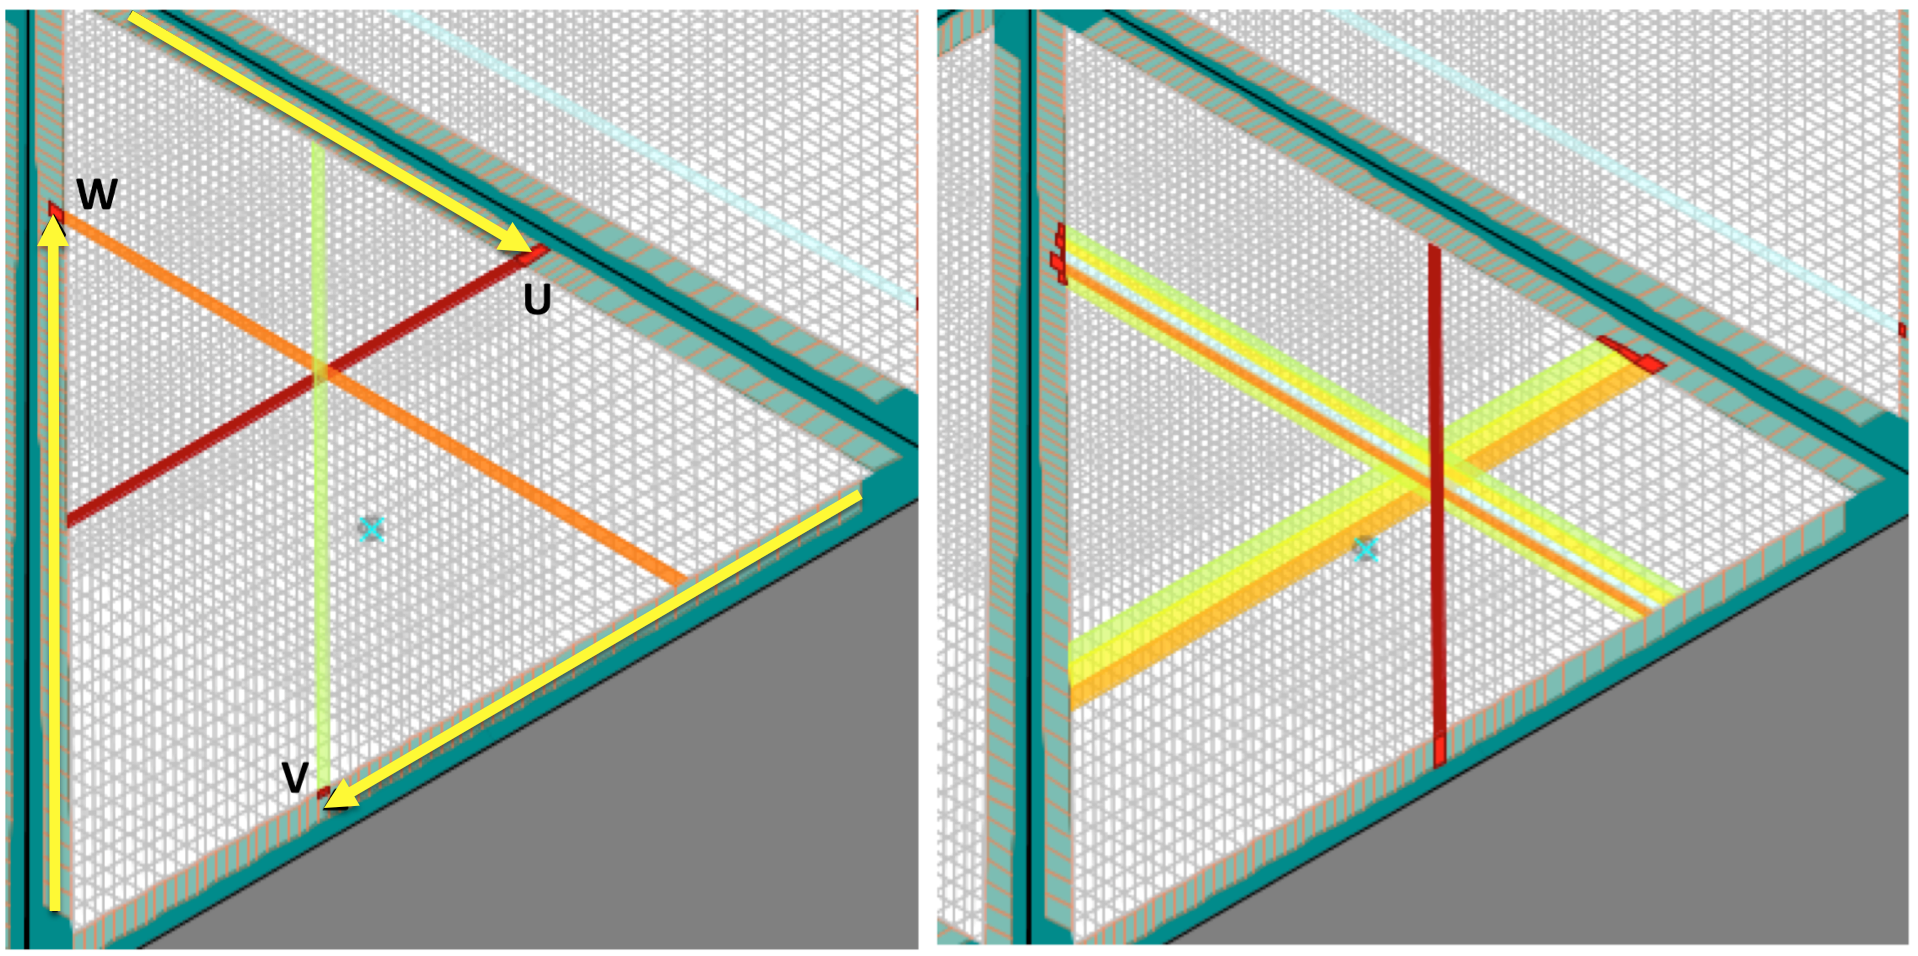
\includegraphics[width=0.95\columnwidth,keepaspectratio]{img/TwoClusters.png}
 \caption{Examples of clusters from cosmic muon triggers.  Desired trajectory (left) is normally incident on the face of PCAL and satisfies the single pixel multiplicity condition (N$_u$=N$_v$=N$_w$=1) in the FPGA pixel trigger.  Event at right shows a more vertical trajectory rejected by this trigger.}
\end{figure}

\begin{figure}[!htb]
 \centering
  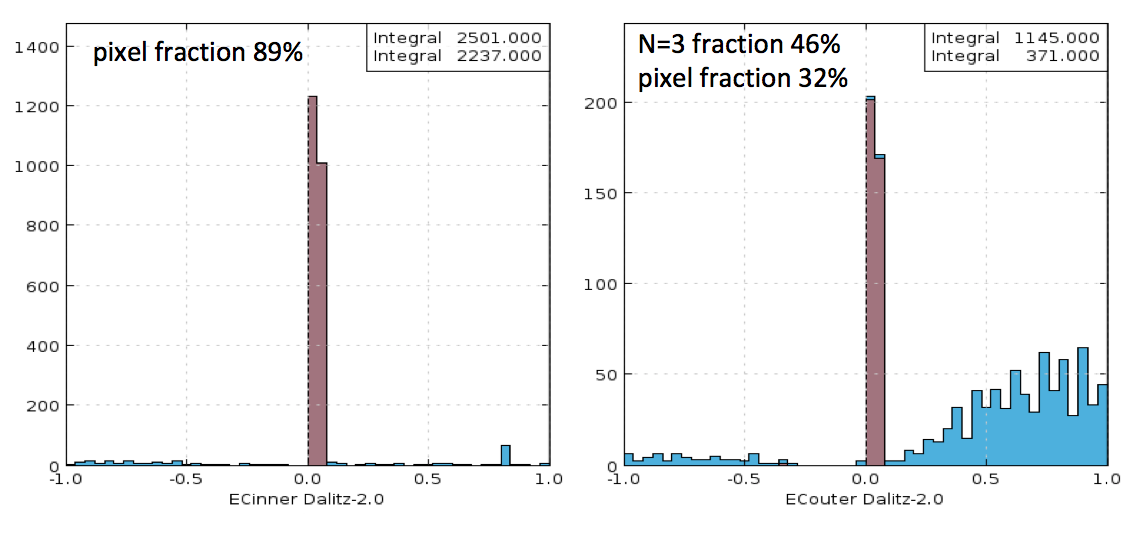
\includegraphics[width=1.0\columnwidth,keepaspectratio]{img/PixelFraction.png}
 \caption{Offline analysis of events which satisfied the pixel trigger on ECINNER calorimeter.  Left plot shows 89$\%$ of ECINNER triggers satisfied the pixel test $dU+dV+dW=2$.  Right plot shows only 14$\%$ of the ECINNER triggers found an ECOUTER event that satisfied both the $N=3$ and pixel test.}
\end{figure}


\subsubsection{Development and Validation of Entire Trigger System with Cosmic Data} 

While the Stage 1 trigger components were validated separately from each other during the development stage, the Stage 2 and Stage 3 components requires the entire system to be assembled to perform validation. Initially those two stages were programmed with simplified alghorithms to test signal propagation and basic trigger system functionality, and only the timing coincidence between different detectors was implemented. Development of Stage 2 and Stage 3 continued during cosmic run operations and later with beam operations, adding a geometrical matches between different detectors and increasing the coincidence logic complexity.

\subsubsection{Development and Validation of Drift Chamber Component of the Trigger System with Beam Data}

%% TO BE WRITTEN

\subsubsection{Trigger System Flexibility and ``Permanent Development'' Mode}

The initial plan was to develop the Trigger System firmware to satisfy all CLAS12 experiments for the entire duration of CLAS12 operation, meaning high (close to 100\%) trigger efficiency and reasonable purity. As the power and flexibility of the trigger system was revealed to the community, additional requirements were requested to improve the system purity, and to include additional physics processes. As a result, the Stage 2 and Stage 3 components of the Trigger System were under constant development during the first year of CLAS12 operation, and the firmware was upgraded and the entire system was validated after every change. After a while, the Trigger System reached the point when relatively small improvements in the trigger purity could only be achieved with significant efforts. At that point the development was declared complete. The nature of the FPGA-based Trigger System allows almost endless improvements, but such ``permanent development'' mode is not practical.
